\documentclass[10pt,a4paper,headsepline,smallheadings]{scrartcl}
\usepackage[utf8]{inputenc}
\usepackage[T1]{fontenc}
\usepackage[ngerman]{babel}
\usepackage{amsmath}
\usepackage{amsthm}
\usepackage{amssymb}
\usepackage{amsfonts}
\usepackage[scaled]{helvet}
\usepackage{amssymb}
\usepackage{multirow}
\usepackage{textcomp}
\usepackage{graphicx}
\usepackage{paralist}
\usepackage{textcomp}
\usepackage{pdflscape} 
\usepackage{marvosym}
\usepackage{float}
\usepackage{siunitx}
\usepackage[siunitx,european,cuteinductors,smartlabels]{circuitikz}
\usepackage{fancyhdr}
\usepackage{pgfplots}
\usepackage{sansmath}
\usepackage{wasysym}

\usetikzlibrary{calc}


\theoremstyle{definition}
\newtheorem{aufgabe}{Aufgabe}


\renewcommand*\familydefault{\sfdefault}
\renewcommand{\arraystretch}{1.1}


\KOMAoptions{parskip=half,DIV=15,fontsize=11pt}
\unitlength1cm
\titlehead{

\begin{center}\begin{tabular}{p{10cm}p{6.8cm}}
\textbf{FH Aachen} & \textbf{FB Maschinenbau und Mechatronik}\\[0.5cm]
\textbf{Modul 86111} &  Prof. Dr. Raphael Pfaff\\
Schienenfahrzeugtechnik I& Sommersemester 2015\\
\end{tabular}

\end{center}
\begin{picture}(0,0)(0,0)\put(17,-23){
\includegraphics[height=5cm]{fh_logo}}\end{picture}
}
\newif\ifuelsg %als slides
%\uelsgtrue
\uelsgfalse
\newif\ifnotuelsg
\ifuelsg\notuelsgfalse\else\notuelsgtrue\fi
\graphicspath{
{../Bilder/Uebungen/}
{../Bilder/Wirkungsplan/}
}

%\titlehead{83105 \hfill Mess-Steuerungs- und Regelungstechnik \hfill Prof. Manfred Enning}
\title{Schienenfahrzeugtechnik I  -- \"Ubung 1}
\date{}
\makeatletter
\let\Title\@title
\let\Author\@author
\makeatother
\pagestyle{fancy}
\fancyhead[LE, LO]{Prof. Dr. Raphael Pfaff}
\fancyhead[RE, RO]{\Title}

\begin{document}
\thispagestyle{empty}
\maketitle
\vspace{-2cm}
% \hyphenation{Abwei-chungen}

\section*{Einf\"uhrung in die Zugdynamik}
\begin{aufgabe}[Zugkraftkennlinie] 
Tragen Sie qualitativ die L\"angskr\"afte der unten gezeigte Z\"uge ein.
\begin{center}
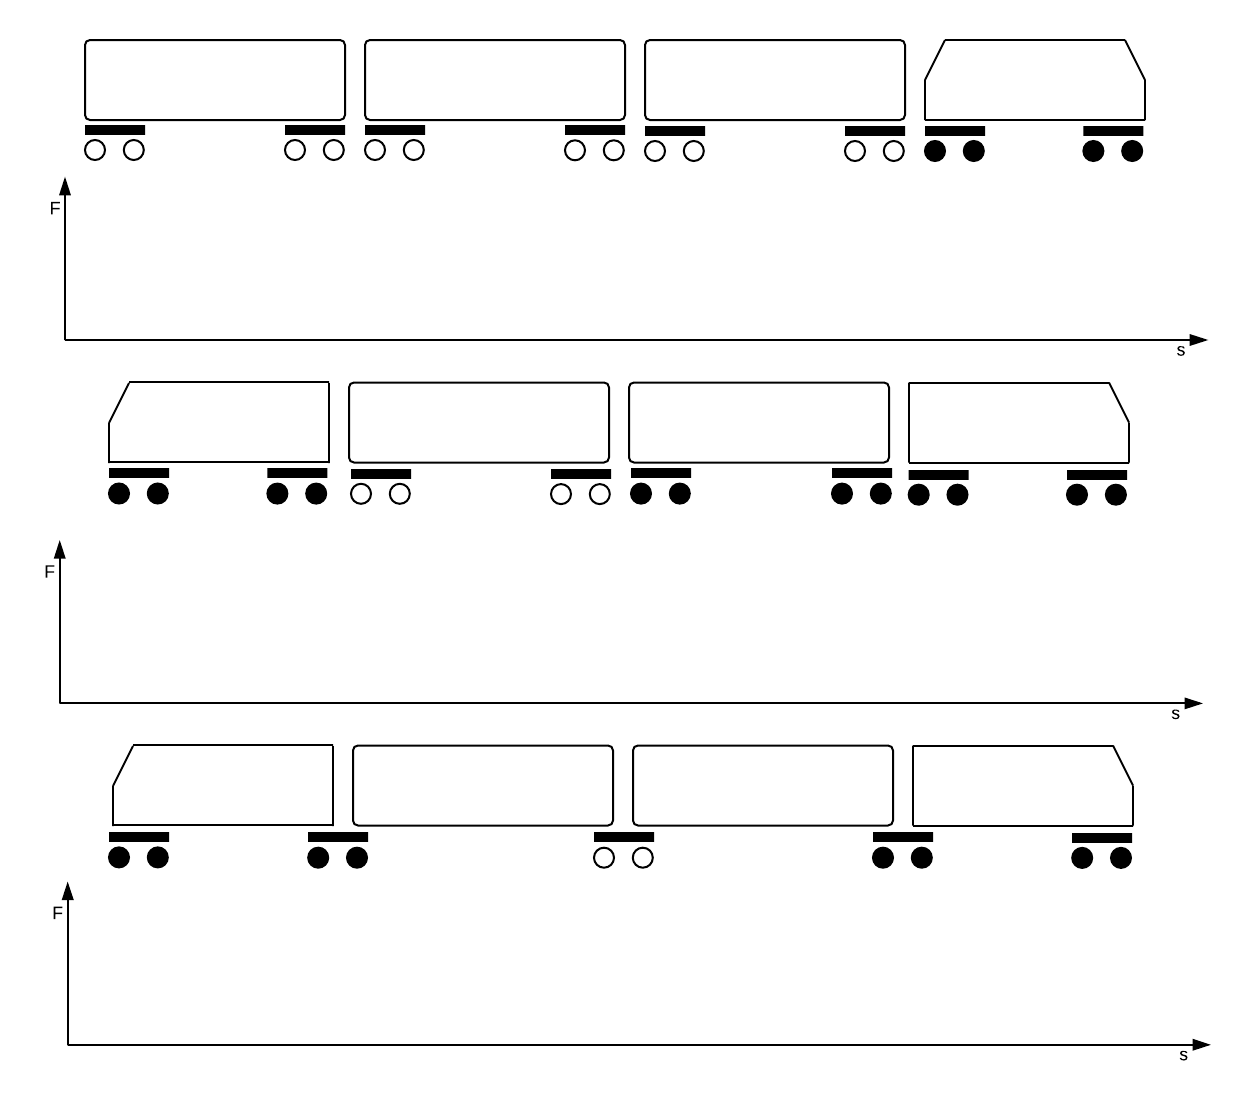
\includegraphics[width = .95\textwidth]{Laengskraefte}
\end{center}
\end{aufgabe}

\begin{aufgabe}[Zugkraftkennlinie] 
Eine Lokomotive der BR 143 der DB AG zieht einen Wagenzug. Die technischen Daten der Fahrzeuge sind:
\begin{itemize}
	\item Triebfahrzeug:
	\begin{itemize}
		\item Masse $m_{L} = 82\, \mathrm{ t}$
		\item Rotierende Masse $m_{DL} = 16\, \mathrm{ t}$
	\end{itemize}
	\item Wagenzug:
	\begin{itemize}
		\item Masse $m_{W} = 500\, \mathrm{t}$
		\item Rotierende Masse $m_{DW} = 24\, \mathrm{t}$
	\end{itemize}
\end{itemize}

\pgfplotsset{width=10 cm}
\begin{center}
	\begin{tikzpicture}
		\begin{axis}[ylabel={$F_{T}/kN$},
		xlabel = {$v/ms^{-1}$}
		%legend, %style={at={(1.5,1)}},
		%anchor=north, legend columns=3},
		%xtick=data
		]]
		\addplot coordinates
			{(0,244) (2.78, 223) (5.55,207) (8.33, 196) (11.11, 189) (13.89, 183) (16.67, 178) (19.44, 174) (22.22, 170) (25, 168) (26.11, 167) (27.78, 144) (29.17, 129) (30.56, 117) (31.94, 107) (33.33, 100)};
			\addplot coordinates
			{(0,11.2) (2.78, 11.5) (5.55, 12.5) (8.33, 13.3) (11.11, 14.8) (13.89, 16.7) (16.67, 18.9) (19.44, 21.6) (22.22, 24.6) (25, 28) (26.11,29.4 ) (27.78, 31.7) (29.17, 33.8) (30.56, 35.9) (31.94, 38.1) (33.33, 40.5)};
			%\addplot coordinates %2%-Gefaelle
			%{(0,111.2) (2.78, 111.5) (5.55, 112.5) (8.33, 113.3) (11.11, 114.8) (13.89, 116.7) (16.67, 118.9) (19.44, 121.6) (22.22, 124.6) (25, 128) (26.11,129.4 ) (27.78, 131.7) (29.17, 133.8) (30.56, 135.9) (31.94, 138.1) (33.33, 140.5)};
		\legend{$F_{T}(v)$, $F_{WZ}(v)$};
		\end{axis}
\end{tikzpicture}
\end{center}

\begin{enumerate}[a)]
\item Zeichnen Sie die Widerstandskurven des Zugverbands (bestehend aus Lokomotive und Wagenzug) f\"ur Streckenneigungen $i_{k} = (1, 2, 4) \%$ in das $F-v$-Diagramm ein. Der Fahrwiderstand des Triebfahrzeugs ist zu vernachl\"assigen.
\item Bestimmen Sie die H\"ochstgeschwindigkeiten $v_{max, k}$ in den jeweiligen Streckenneigungen.
\item Bestimmen Sie das Beschleunigungsverm\"ogen des Zugverbands in der Ebene und in 1\% Streckenneigung f\"ur $v = 90\, \mathrm{km/h}$.
\item Bestimmen Sie die kinetische Energie des Zugverbands bei $v = 120 \, \mathrm{km/h}$ und bestimmen Sie f\"ur einen mittleren Fahrwiderstand von $F_{W,m} =20 \, \mathrm{kN}$ in einer Steigung von 1\% die Steigh\"ohe bis v = 0 gilt.
\end{enumerate}
\end{aufgabe}

\section*{Einf\"uhrung in die Spurf\"uhrung}
\begin{aufgabe}[Erarbeitung Klingel'sche Formel] 
Bearbeiten Sie folgende Aufgabe in Kleingruppen (2-3 Studierende).

Betrachten Sie einen Einzelradsatz mit konischem Radprofil, zun\"achst in Querrichtung verschoben:
\begin{center}
	\begin{tikzpicture}[scale = 0.8]
	\draw[ultra thick, draw = red!70!black] (-2,-.4) -- (11,-.4){};
	\draw[ultra thick, draw = red!70!black] (-2,3.1) -- (11,3.1){};
	\draw[<->,thick] (10.5,-.4) -- (10.5,3.1);
	\node[right] at (10.5,1.35) {$2b$};
	\path[fill = blue!30, opacity = 0.5] (-1,-1) -- (4,-1) -- (4,4) --(-1,4) -- (-1,-1);
	\draw[thick, fill = gray!30] (0,3) -- (3,3) -- (2.8,3.5) -- (0.2,3.5) -- (0,3) {}; 
	\draw[thick, fill = gray!30] (1.3,0) -- (1.7,0) -- (1.7,3) -- (1.3,3) -- (1.3,0) {}; 
	\draw[thick, fill = gray!30] (0,0) -- (3,0) -- (2.8,-0.5) -- (0.2,-0.5) -- (0,0) {}; 
	\draw[->,thick] (-3,1.5) -- (-1.5,1.5);
	\node[above] at (-2.25,1.5) {$v$};
	\path[fill = green!30, opacity = 0.5] (5,-1) -- (10,-1) -- (10,4) --(5,4) -- (5,-1);
	\draw[thick, fill = gray!30, rotate around={-4:(7.5,1.5)}] (6,3) -- (9,3) -- (8.8,3.5) -- (6.2,3.5) -- (6,3) {}; 
	\draw[thick, fill = gray!30, rotate around={-4:(7.5,1.5)}] (7.3,0) -- (7.7,0) -- (7.7,3) -- (7.3,3) -- (7.3,0) {}; 
	\draw[thick, fill = gray!30, rotate around={-4:(7.5,1.5)}] (6,0) -- (9,0) -- (8.8,-0.5) -- (6.2,-0.5) -- (6,0) {}; 
	\draw[draw = blue!80, fill = blue!50] (7.63,0.5) -- (7.71,1.5) -- (7.71,0.5);
	\node[right] at (7.71,0.7) {\color{blue!80!black} $\varphi$};
	\draw[->,thick] (3.75,1.5) -- (5.25,1.5);
	\node[above] at (4.5,1.5) {$x$};
	\draw[->,thick] (3.75,1.5) -- (3.75,3);
	\node[right] at (3.75,2.25) {$y$};
	\draw[->,thick] (5.25,1.6) arc [->,start angle=0, end angle=90, radius=1.4];
	\node[right] at (5.1,2.25) {$\varphi$};
	\end{tikzpicture}
\end{center}

\begin{enumerate}
	\item Bestimmen Sie die Quergleitgeschwindigkeit abh\"angig von $v$ und $\varphi$.
	\begin{itemize}
		\item Vereinfachen Sie so, dass die Abh\"angigkeit von $\varphi$ linear ist.
		\end{itemize}
	\item Differenzieren Sie, um die Querbeschleunigung zu erhalten. Annahme: $v$ konstant.
	\item Bestimmen Sie die Winkelgeschwindigkeit $\dot{\varphi}$ des Radsatzes um die Hochachse abh\"angig von
	\begin{itemize}
		\item Rollradiendifferenz $\triangle r$,
		\item halbem Radstand $b$ sowie 
		\item Winkelgeschwindigkeit des Radsatzes $\omega$.
	\end{itemize}
	\item Vereinfachen Sie f\"ur kegelf\"ormige Rads\"atze $\triangle r$.
	\item Leiten Sie die homogene lineare Differenzialgeichung der Bewegung in $y$-Richtung aus den oben gefundenen Beziehungen her.
	\begin{itemize}
		\item Welche Eigenschaften hat diese Differenzialgleichung?
		\item Welche (wichtigen) Aspekte haben Sie vernachl\"assigt?
	\end{itemize}
	\item Bestimmen Sie Eigenkreisfrequenz und die Wellenl\"ange der Bewegung.
	\begin{itemize}
		\item Welche Beobachtungen k\"onnen Sie machen?
	\end{itemize}
\end{enumerate}


\end{aufgabe}

\section*{Kraftschluss und Schlupf}
\begin{aufgabe}[Kraftschlussausnutzung]
Ein dreiteiliger Triebzug wird beschleunigt und gebremst. Die Daten des Triebzugs sind:
\begin{itemize}
	\item Achsformel Bo' Bo' + 2' 2' + Bo' Bo'
	\item $m_{W,i} = 40 \mathrm{t}$
	\item Zus\"atzliche rotierende Massen (anteilig von $m_{W,i}$):
	\begin{itemize}
		\item Treibachsen $\rho_{T} = 0{,}15$
		\item Laufachsen $\rho_{L} = 0{,}08$
	\end{itemize} 
	\item Beschleunigungsverm\"ogen: $a_{max} = 1{,}5 \frac{\mathrm{m}}{\mathrm{s}^2}$
	\item Verz\"ogerung der Schnellbremse: $b_{max} = 1{,}2 \frac{\mathrm{m}}{\mathrm{s}^2}$
\end{itemize} 

Bestimmen Sie:
\begin{enumerate}[a)]
\item Treibachsbremskr\"afte (Lauf- und Treibachsen) und Kraftschlussausnutzung w\"ahrend einer Schnellbremsung
\item Treibachszugkraft und Kraftschlussausnutzung w\"ahrend der maximalen Beschleunigung
\item Die Bremse muss an zwei Drehgestellen (1 Laufdrehgestell, 1 Triebdrehgestell) auf Grund eines Fehlers abgesperrt werden. Bestimmen Sie die verbleibende Verz\"ogerung sowie die Kraftschlussausnutzung, f\"ur die die Bremsleistung konstant gehalten werden k\"onnte.
\end{enumerate}
\end{aufgabe}
\vspace{0.5cm}
\begin{aufgabe}
Ein G\"uterwagen (Masse leer $m_{L} = 30 \mathrm{t}$, Masse unter maximaler Beladung $m_{B} = 80 \mathrm{t}$, rotierende Masse $m_{R} = 3{,}2 \mathrm{t}$) erreicht eine maximale Verz\"ogerung $b_{max} = 0{,}7 \frac{\mathrm{m}}{\mathrm{s}^2}$.
Bestimmen Sie:
\begin{enumerate}[a)]
\item Treibachsbremskraft und Kraftschlussausnutzung w\"ahrend einer Schnellbremsung des beladenen Wagens
\item Kraftschlussausnutzung w\"ahrend einer Schnellbremsung des unbeladenen Wagens unter der Annahme einer konstanten Bremskraft am Radumfang
\item Treibachsbremskraft des unbeladenen Wages f\"ur eine Kraftschlussausnutzung von $0{,1}$.
\end{enumerate}

\end{aufgabe}

\section*{Bremskurven}
\begin{aufgabe}[Bremsarten]
Ein zweistufiges Bremsmodell nutzt folgende Stufen, um einen Bremsprozess mit Füllzeit $t_f$ und Verzögerung $\bar{a}$ zu modellieren:
\begin{itemize}
	\item Konstantfahrt für eine Dauer von $\frac12 t_f$
	\item Konstante Verzögerung $\bar{a}$ von $\frac12 t_f$ bis zum Stillstand des Fahrzeugs
\end{itemize}
\begin{enumerate}[a)]
\item Skizzieren Sie die Bremskurven im v-s-Diagramm, wobei der Unterschied zwischen den Bremsarten herausgestellt werden soll.
\item Welchen Einfluss hat eine l\"angere F\"ullzeit auf
\begin{itemize}
	\item die zul\"assige H\"ochstgeschwindigkeit im Vorsignal-Hauptsignal-System?
	\item die L\"angsdruckkr\"afte w\"ahrend einer Bremsung?
\end{itemize}
\end{enumerate}
\end{aufgabe}
\vspace{.5cm}
\begin{aufgabe}[L\"angsdruckkr\"afte]
In einem Zugverband, der ansonsten frei von L\"angszug- und -druckkr\"aften ist, befinden sich zwei Gelenktragwagen der Bauart Sggrss (L\"uP = 27 m). Die verbauten Steuerventile der Wagen liegen ung\"unstig verteilt im Rahmen der Toleranzen gem\"a{\ss} UIC 540 in Bremsstellungen G bzw. P , sodass im vorderen Wagen die k\"urzeste und im hinteren Wagen die l\"angste F\"ullzeit erreicht wird. Bestimmen Sie die auftretenden L\"angsdruckkr\"afte unter folgenden Annahmen:
\begin{itemize}
	\item Durchschlagsgeschwindigkeit $v_{SB} = 250 \frac{\mathrm{m}}{\mathrm{m}}$
	\item Linearer Aufbau der Bremskraft von $0$ auf $F_{B, max}$ innerhalb der F\"ullzeit $t_{f}$
	\item Masse der Wagen $m_{W} = 60 \mathrm{t}$, rotierende Masse $m_{D} = 2{,}5 \mathrm{t}$
	\item Bremskraft am Radumfang $F_{B} = 60 \mathrm{kN}$
\end{itemize}
\end{aufgabe}

\section*{Fahrwiderstand}
\begin{aufgabe}[Fahrwiderstand nach Strahl und Sauthoff]
\begin{enumerate}[a)]
\item Berechnen Sie die ben\"otigte Energie f\"ur je $s = 100 \mathrm{km}$ Streckenfahrt mit $v_{max}$:
\begin{itemize}
		\item Gemischter G\"uterzug, $v_{max} = 80 \frac{\mathrm{km}}{\mathrm{h}}$, $m_{W} = 4000 \mathrm{t}$
		\begin{itemize}
		\item Widerstandsgleichung nach Strahl:
		\begin{equation}
		\label{Eq:Strahl}
			f_{WW} = 1{,}6 \permil +  5{,}7 \permil \left( \frac{v}{100 \frac{\mathrm{km}}{\mathrm{h}}} \right)^2
		\end{equation}
		\end{itemize}
		\item Reisezug, $v_{max} = 160 \frac{\mathrm{km}}{\mathrm{h}}$, $m_{W} = 350 \mathrm{t}$, $n_{W} = 7$
 		\begin{itemize}
		\item Widerstandsgleichung nach Sauthoff:
		\begin{equation}
		\label{Eq:Sauthoff}
			f_{WW} = 1{,}6 \permil + 0{,}25 \permil \left( \frac{v}{100 \frac{\mathrm{km}}{\mathrm{h}}} \right) + 
			\frac{683 \mathrm{N}(2{,}7 + n_{W}) }{m_{W} g} \left( \frac{v+ 12 \frac{\mathrm{km}}{\mathrm{h}}}{100 \frac{\mathrm{km}}{\mathrm{h}}} \right)^2
		\end{equation}
		\end{itemize}
		\end{itemize}
\item Berechnen Sie die ben\"otigte Energie f\"ur das Beschleunigen der Z\"uge auf $v_{max}$ unter Ber\"ucksichtigung des Fahrwiderstands gem\"a{\ss} der Gleichungen \eqref{Eq:Strahl} bzw. \eqref{Eq:Sauthoff} sowie einer konstanten Beschleunigung von
\begin{itemize}
		\item $a = 0{,}1 \frac{\mathrm{m}}{\mathrm{s}^2}$ f\"ur den G\"uterzug
		\item $a = 0{,}3 \frac{\mathrm{m}}{\mathrm{s}^2}$ f\"ur den Personenzug
		\end{itemize}
\end{enumerate}
Der Widerstand des Triebfahrzeugs ist zu vernachl\"assigen.
\end{aufgabe}

\section*{L\"angsdynamik}

\begin{aufgabe}[Massenband/Massenpunktmodell]
Ein siebenteiliger Triebzug ($m_{w} = 50 \, \mathrm{t}$, $l_{w} = 25 \, \mathrm{m}$) f\"ahrt auf einer Strecke, die der Vorschrift 
 \begin{equation*}
h(x) = 
\begin{cases}
 0, \quad x < 5000 \\
 - 100 \cos \frac{x-5000}{5000} + 100, \quad x \geq 5000
\end{cases}
\end{equation*}
entspricht. Hierbei wird die Position der Zugspitze $x$ in $\mathrm{m}$ gemessen.
\begin{enumerate}[a)]
\item Bestimmen Sie die maximale Streckenneigung $i_{max}$ der Strecke.
\item Bestimmen Sie den Punkt, an dem $E_{pot} > 0$ gilt im Massenband- bzw. Massenpunktmodell.
\item Bestimmen Sie f\"ur $x = 7000$ die Neigungswiderstandskraft des Zugverbands, jeweils im Massenband- bzw. Massenpunktmodell.
\end{enumerate}

\end{aufgabe}
\vspace{.5cm}
\begin{aufgabe}[Kuppelsto{\ss}/Crash]
Ein dreiteiliger Metro-Triebzug ($m_{w} = 50 \, \mathrm{t}$) soll mit einer automatischen Mittelpufferkupplung ausgestattet werden, die Kuppeln mit $v = 4 \frac{\mathrm{km}}{{h}}$ zul\"asst. Der maximale Hub der Frontkupplung sei auf $s_{max} = 50 \mathrm{mm}$ begrenzt, die Zwischenkupplungen seien starr. Das stehende Fahrzeug ist w\"ahrend des Kuppelns mit der selbstt\"atigen Bremse gebremst.
\begin{enumerate}[a)]
\item Welche Kraft muss \"uber den Verz\"ogerungsweg durchschnittlich herrschen, um die dieses Kuppeln zuzulassen? Hierbei sei die Energie ausschlie{\ss}lich \"uber die Kupplung verzehrt.
\item Was geschieht mit dem stehenden Fahrzeug?
\item Welche Verz\"ogerung herrscht unter dem Annahmen von Aufgabe a) im fahrenden Fahrzeug?
\item Bei einem Crash mit einem baugeichen Fahrzeug mit $v = 18 \frac{\mathrm{km}}{{h}}$ stehen Energieverzehrelemente mit einem Hub von $s = 200 \mathrm{mm}$ zur Verf\"ugung. Welche Verz\"ogerung und welche Kraft stellt sich ein?
\end{enumerate}
\end{aufgabe}


\end{document}